\documentclass{beamer}

\usetheme{Marburg}

\title{Maintainable Embedded Linux Solutions}
\author{Thomas Irgang \and Simone Weiß}
\institute{EASTERHEGG 2024 - RABBIT PROTOTYPING}
\date{March 31, 2024}
\titlegraphic{
    
\includegraphics[width=2cm]{assets/logo.png}
}

\newcommand\pro{\item[$+$]}
\newcommand\con{\item[$-$]}

\begin{document}

\begin{frame}
    \titlepage
\end{frame}

\section{Why Linux?}

\begin{frame}{Do I need Linux for my project?}
	\begin{tabular}{cccc}
	&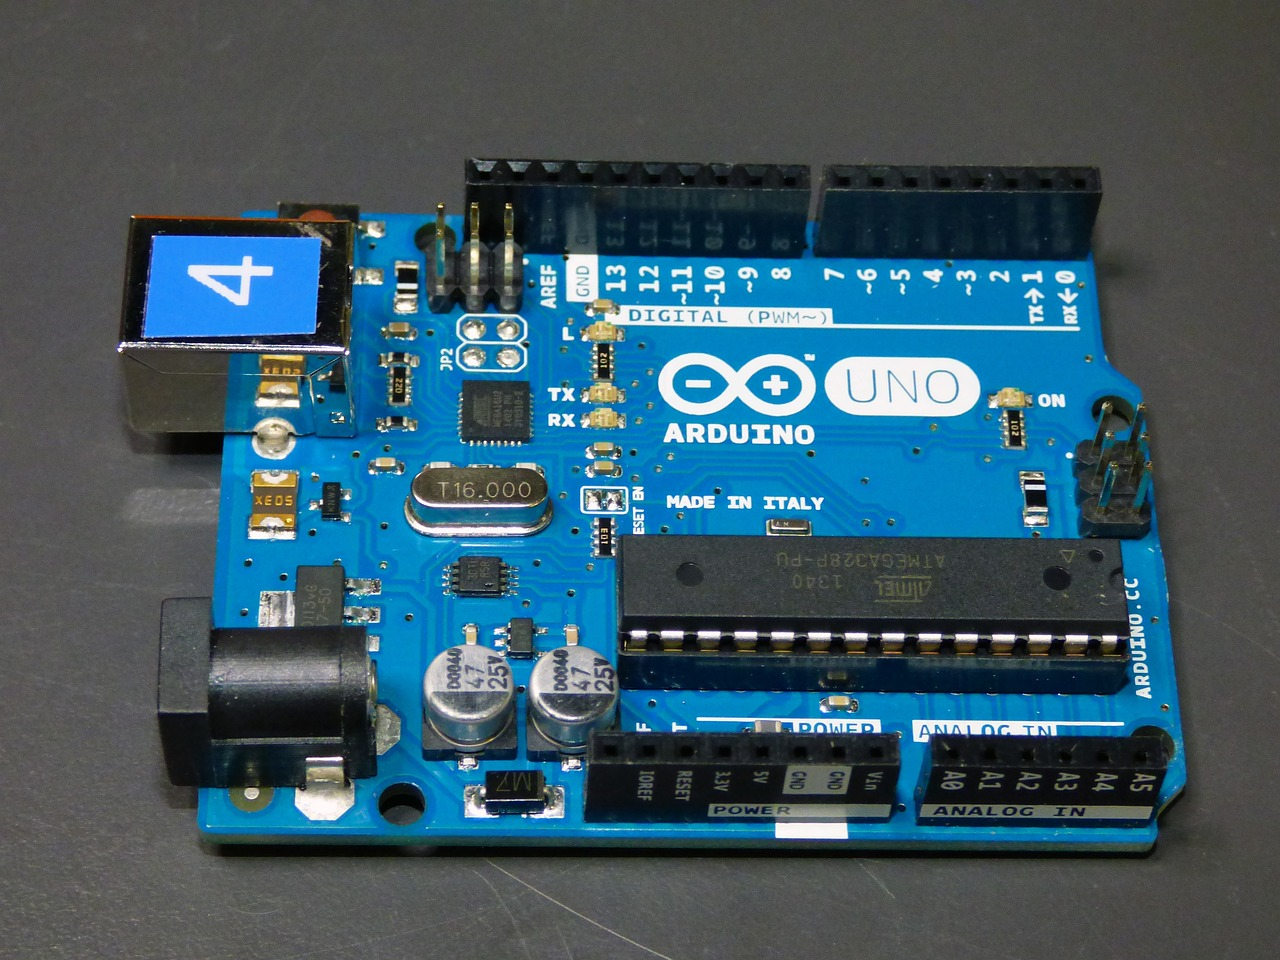
\includegraphics[width=1.9cm]{assets/Pixabay_Arduino_integrated-circuit-441289_1280.jpg} &
	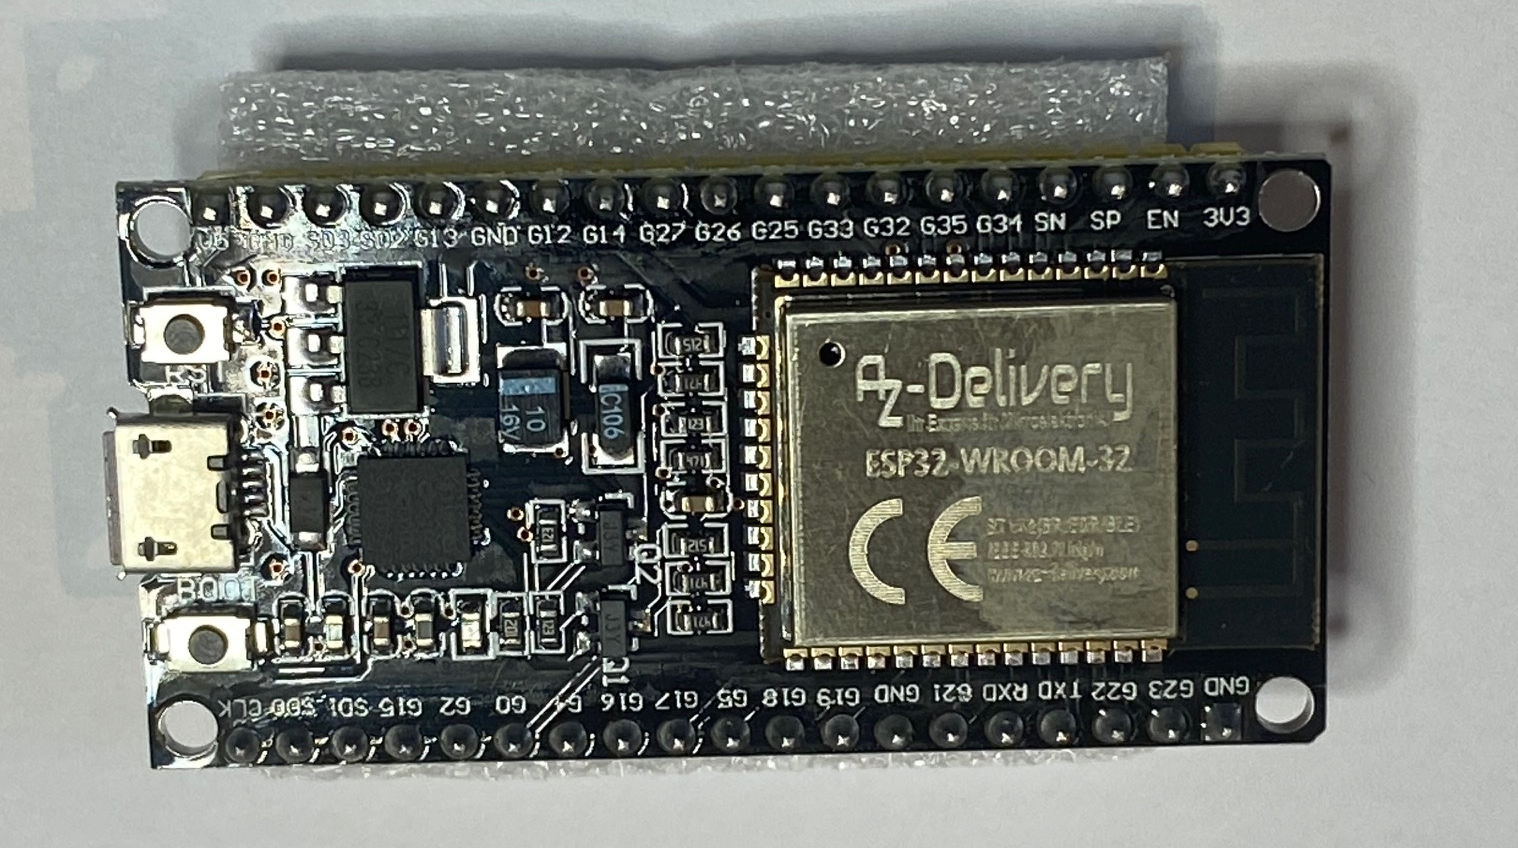
\includegraphics[width=1.9cm]{assets/ESP32.png} & 
	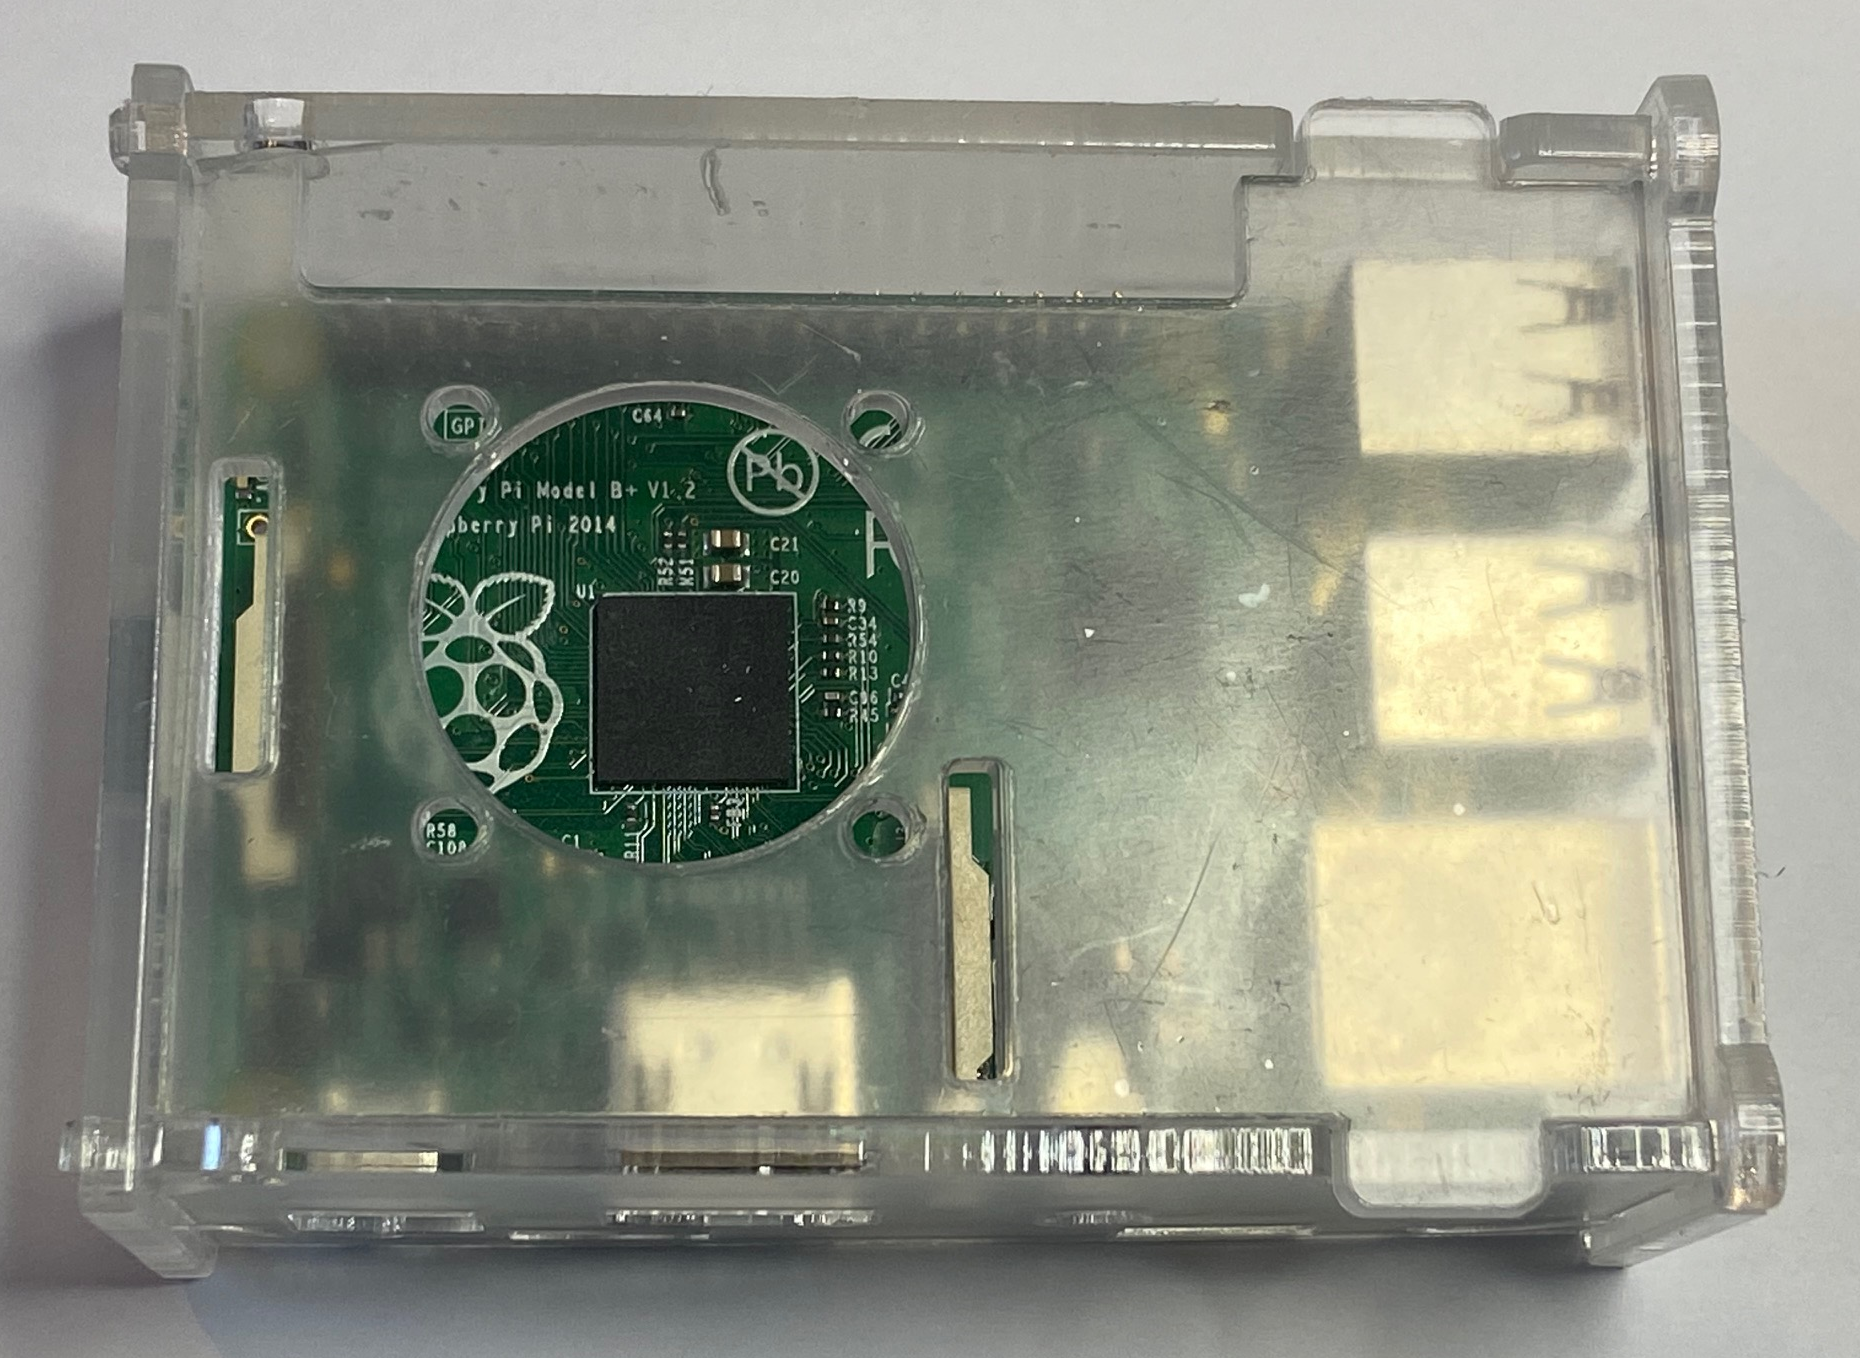
\includegraphics[width=1.9cm]{assets/Raspberry_Pi.png} \\
	&\textbf{Arduino} & \textbf{ESP32 FreeRTOS} & \textbf{SBC Linux} \\
	real-time & + &  + & - \\
	energy & + & o & - \\
	UI & - & - & + \\
	IO & - & o & + \\
	CPU & - & o & + \\
	\end{tabular}
\end{frame}

\begin{frame}{What's the life-time of my project?}
	\begin{columns}
    \column{0.33\textwidth}
        \centering
        \textbf{Experiment}
        \begin{itemize}
        		\item few months
        		\item no maintenance
        		\item some reusability
        \end{itemize}
    \column{0.33\textwidth}
        \centering
        \textbf{Media-Center}
        \begin{itemize}
        		\item some years
        		\item typical IT distribution maintenance
        		\item no reusability needed
        \end{itemize}
    \column{0.34\textwidth}
        \centering
        \textbf{Home Automation}
        \begin{itemize}
        		\item more than 15 years
        		\item maintenance and upgrades
        		\item reusability for mid-term upgrade needed
        \end{itemize}
    \end{columns}
\end{frame}

\section{Building an embedded Linux solution}

% Raspberry Pi approach

% Yocto / Buildroot

% Elbe / Debos / Kiwi

% comp

\section{Remixing an embedded Linux}

% comp Elbe / Debos / Kiwi




\end{document}
